\part[author={\protect\insertauthor},label={chap:runtime_environments}]{Run-time Environments}

\begin{graphicspathcontext}{{./chapters/chapter5/imgs/auto/},{./chapters/chapter5/imgs/raw/},{./chapters/chapter1/imgs/auto/}}
\begin{bibunit}[apalike]

\tableofcontentslide

\section{Introduction}
\sectiontableofcontentslide

\begin{rightlawnframe}<13>{Run-time Environments}{runtime-environment-introduction}
	\putat*(340,-197){\includeanimatedfigure[width=2.5cm]{compiler_structure}}
	Compiler implements abstractions from source language \\[.2cm]
	\emph{Compiler cooperates with operating system and other systems software to support these abstracts on the target machine} \\[.2cm]
	Compiler creates and manages a \Emph{run-time environment} in which it assumes its target programs are being executed
\end{rightlawnframe}

\begin{frame}{Content of this Chapter}
	\fancybox{Heap}{Management of dynamic memory allocation}{heap-icon}{}
	\hfill
	\fancybox{Stack}{Management of static memory allocation}{stack-icon}{}
	\hfill
	\fancybox{Dynamic Memory Deallocation}{Management of deallocation}{deallocation-icon}{}
\end{frame}

\section{Data Storage}
\sectiontableofcontentslide

\begin{frame}{Storage Organization}
	\begin{rightarrowsequence}
		\arrow[bg=CIADlightgray,fg=black]{
			Target program runs in its \alert{own logical address space} in which each value has a location
		}
		\arrow[bg=CIADdarkgray]{
			Operating system maps the logical addresses into physical addresses
		}
		\arrow[bg=CIADlightgray,fg=black]{
			\alert{Virtual machine} represents the operating system and the target machine into an abstract and platform-independent machine
		}
	\end{rightarrowsequence}
\end{frame}

\sidecite{Randell.1964}
\begin{frame}[t]{Structure of the Logicial Address Space}
	\alertbox*{
		In the run-time environment, logical address space has a structure; typically:
	}
	\vspace{.2cm}
	\begin{columns}
		\begin{column}{.3\linewidth}
			\raisebox{-.5\height}{\includeanimatedfigure[width=\linewidth]{address_space_structure}}
		\end{column}
		\begin{column}{.7\linewidth}\begin{small}
				\only<2>{\begin{itemize}
						\item Compiler places executable target code in a statically determined area, named \emph{Code}
						\item Contains binary representations of the instructions to execute
						\item Format of the code depends on the target machine: Intel binary assembler, byte code\dots
				\end{itemize}}
				\only<3>{\begin{itemize}
						\item Size of some program data may be known at compile time
						\item Area where these data are stored in named \emph{Static Data}, usually put just after the Code area
						\item \inlineexamples{string literals, global constants and variables, information related to garbage collection\dots}
						\item Address of static data is directly put in the code
				\end{itemize}}
				\only<4>{\begin{itemize}
						\item \alert{Stack} is used to store data structures, named \alert{activation records}
						\item Activation records are generated during the procedure/function calls (explained later)
						\item Each record contains the status of the machine: ordinal counter, machine registers, and data whose lifetimes are the same as the activation time (usually local variables)
				\end{itemize}}
				\only<5>{\begin{itemize}
						\item Many languages allow the programmer to allocates and deallocates data under program control (malloc, new\dots)
						\item \alert{Heap} is used to manage this kind of long-lived data
				\end{itemize}}
				\only<6>{\begin{itemize}
						\item Heap and the stack are growing up and consume the \alert{free memory space} between them
						\item When the stack cannot grow up, the classical ``stack overflow'' error is fired
						\item When the heap cannot grow up, the classical ``out of memory'' error is fired
				\end{itemize}}
			\end{small}
		\end{column}
	\end{columns}
\end{frame}

\begin{frame}{Static vs. Dynamic Storage Allocation}
	\hiconbox{
		{\larger\emph{Static Storage Allocation}}
		\newline\newline
		Made \alert{by the compiler} looking only at the text of the program, not at what the program does when it executes \newline
		Allocation is usually done on the static data area
	}{static-allocation-icon}
	\vspace{1cm}
	\hiconbox{
		{\larger\emph{Dynamic Storage Allocation}}
		\newline\newline
		Made only \alert{while the program is running} \newline
		Allocation may be on the stack or the heap (see next slide)
	}{dynamic-allocation-icon}
\end{frame}

\sidecite{Randell.1964}
\begin{frame}[t]{{Dynamic Storage Allocation} Strategies}
	\hiconbox{
		\begin{minipage}[b]{\linewidth}\begin{block}{Stack Storage}
			\begin{itemize}
				\item Local-scope names are allocated space \alert{on a stack}
				\item Stack serves the normal call/return policy for procedures
			\end{itemize}
		\end{block}\end{minipage}
	}{stack-icon}
	\vspace{.25cm}
	\hiconbox{
		\begin{minipage}[b]{\linewidth}\begin{block}{Heap Storage}
			\begin{description}
				\item Data that may outlive the call to the procedure that created it is usually allocated \alert{on a ``heap''} of reusable storage.
				\item The heap is an area of virtual memory that allows data to obtain and release storage.
				\item[Garbage collection] the run-time environment detects useless data in heap and releases them.
			\end{description}
		\end{block}\end{minipage}
	}{heap-icon}
\end{frame}

\section{Stack management}
\sectiontableofcontentslide

\subsection{Stack allocation}

\subsubsection{General Principles}
\subsubsectiontableofcontentslide

\sidecite{Randell.1964}
\begin{frame}{Stack Allocation}
	\alertbox*{
		Compilers that use procedures, functions, or methods as units manage a part of their run-time memory as a stack
	}
	\vspace{.5cm}
	\hiconbox{
		Procedure will be used as a generic term for procedure, function and method
	}{note-icon}
	\vspace{.5cm}
	\begin{rightarrowsequence}
		\arrow[bg=CIADlightgray,fg=black]{
			\textcolor{CIADgreen}{When procedure is called} \\
			Space for its local variables is pushed on stack
		}
		\arrow[bg=CIADdarkgray]{
			\textcolor{CIADlightgreen}{When procedure terminates} \\
			Space is popped from stack
		}
		\arrow{
			Procedure activation \\ $\equiv$ \\ Procedure call
		}
	\end{rightarrowsequence}
\end{frame}

\begin{frame}[fragile]{{Nested Activation} in Time}
	\begin{small}
		\alertbox{Stack allocation would not be feasible if procedure calls did not nest in time}
		\begin{columns}
			\begin{column}{.5\linewidth}
				If an activation of procedure \ccode{p} calls procedure \ccode{q}, then that activation of \code{q} must end before the activation of \ccode{p} can end \\[.2cm]
				\pgfuseimage{nested-activation}
			\end{column}
			\begin{column}{.5\linewidth}
				\begin{lstlisting}[style=lststyle-c,basicstyle=\tiny]
int a[11];
void readArray() {
  int i; // read and fill a
}
int partition(int m, int n) {
  // let v, a[m..p-1] < v, a[p]=v, a[p+1..n] >= v
  // return p
}
void quicksort(int m, int n) {
  int i;
  if (n>m) {
    i = partition(m,n);
    quicksort(m,i-1);
    quicksort(i+1,n);
  }
}
main() {
  readArray();
  a[0] = -9999;
  a[11] = 9999;
  quicksort(1,9);
}
				\end{lstlisting}
			\end{column}
		\end{columns}
	\end{small}
\end{frame}

\begin{frame}[t]{Termination of Nested Activation}
	\begin{small}
	\alertbox*{Three common cases when \code{p} calls \code{q}}
	\vspace{.1cm}
	\hiconbox{
		\textcolor{CIADgreen}{Normal:} activation of \code{q} terminates normally \newline
		Then in many languages, control resumes just after the point of \code{p} at which the call to \code{q} was made
	}{procedure-normal-run}
	\vspace{.1cm}
	\hiconbox{
		\textcolor{CIADgreen}{Abort:} activation of \ccode{q}, or some procedure called by \ccode{q}, either directly or indirectly, aborts \newline
		\ccode{p} ends simultaneously with \code{q}
	}{procedure-abort-run}
	\vspace{.1cm}
	\hiconbox{
		\textcolor{CIADgreen}{Exception:} activation of \ccode{q} terminates because of an exception that \ccode{q} cannot handle \newline
		Procedure \ccode{p} may handle the exception: activation of \ccode{q} has terminated but \ccode{p} continues (not necessary where \ccode{q} was called) \newline
		If \ccode{p} cannot handle the exception, then this activation of \ccode{p} terminates at the same time as the activation of \ccode{q}, and exception will be handled by some other open activation of a procedure
	}{procedure-exception-run}
	\end{small}
\end{frame}

\subsubsection{Activation tree}
\subsubsectiontableofcontentslide

\begin{frame}{Activation Tree}
	\begin{definition}
		Activations of procedures during the running is represented by a tree, where:
		\begin{description}
			\item[Node] an activation
			\item[Root Node] activation of the ``main'' procedure
			\item[Child Node] activations of the procedures called by the activation represented by the parent node \\
			The order of the children (from left to right) is the order of the activations
		\end{description}
	\end{definition}
\end{frame}

\figureslide{Example of Activation Tree}{activation_tree_example}

\subsubsection{Control stack and activation record}
\subsubsectiontableofcontentslide

\begin{frame}{{Control Stack} and Activation Record}
	\begin{definitionblock}{Activation Record}
		List of information that are describing a procedure activation
	\end{definitionblock}
	\vspace{.25cm}
	\begin{definitionblock}{Control Stack}
		Stack used for managning the procedure calls and returns \\
		Each live activation has an \emph{activation record} (or frame) on the control stack \\
		
	\end{definitionblock}
	\vspace{.25cm}
	\begin{itemize}
		\item Entire sequence of activation records on the stack is the path in the activation tree to the activation where control currently resides
		\item \emph{Latter activation has its record at the top of the stack}
	\end{itemize}
\end{frame}

\figureslide{Example of Control Stack}{control_stack_example}

\begin{frame}{Structure of the Activation Record}
	\alertbox*{Contents of activation records vary with the language being implemented; typically:}
	\vspace{1cm}
	\begin{columns}
		\begin{column}{.3\linewidth}
			\raisebox{-.5\height}{\includeanimatedfigure[width=\linewidth]{activation_record_structure}}
		\end{column}
		\begin{column}{.7\linewidth}\begin{small}
				\only<2>{\begin{itemize}
						\item Temporary values \tactext{\t{k}}
						\item Arising from the evaluation of expressions
						\item Only in case where the temporaries cannot be held in processor registers
				\end{itemize}}
				\only<3>{\begin{itemize}
						\item Local data declared in activated procedure
				\end{itemize}}
				\only<4>{\begin{itemize}
						\item Information about the state of the machine just before the call to the procedure
						\item It typically includes:
						\begin{description}
							\item[Return address] value of the ordinal counter to which the called procedure must return
							\item[Registers] Contents of registers that were used by the calling procedure and that must be restored when the return occurs
						\end{description}
				\end{itemize}}
				\only<5>{\begin{itemize}
						\item ``Access link'' to locate data needed by the called procedure found elsewhere (in another activation record\dots)
				\end{itemize}}
				\only<6>{\begin{itemize}
						\item ``Control link'' is pointing to the activation record of the caller
				\end{itemize}}
				\only<7>{\begin{itemize}
						\item Space for the return value of the called function, if any
						\item Not all called procedures return a value
						\item We may prefer to place that value in a register for efficiency
				\end{itemize}}
				\only<8>{\begin{itemize}
						\item Actual parameters are given by the caller and used by the callee procedure
						\item Commonly, these values are not placed in the activation record but rather in registers, when possible
				\end{itemize}}
			\end{small}
		\end{column}
	\end{columns}
\end{frame}

\subsubsection{Calling sequence}
\subsubsectiontableofcontentslide

\sidecite{Johnson.1981}
\begin{frame}{Introduction to Calling and Return Sequences}
	\begin{definitionblock}{Calling Sequence}
		A code that allocates an activation record on the stack and enters information into its fields
	\end{definitionblock}
	\vspace{.25cm}
	\begin{definitionblock}{Return Sequence}
		A code that deallocates an activation record from the stack and restores the state of the machine
	\end{definitionblock}
	\vspace{.25cm}
	\alertbox{
		Calling sequences and the layout of activation records may differ greatly, \newline
		even among implementations of the same language
	}
\end{frame}

\sidecite{Randell.1964}
\begin{frame}[t]{Principles of the Calling Sequences}
	\putat*(230,-180){\includeanimatedfigure[width=.4\paperwidth]{calling_sequence_principles}}
	\only<1>{\begin{enumerate}
			\item \emph{Values communicated between caller and callee procedures are generally placed at the beginning of the callee activation record}
	\end{enumerate}}
	\only<2>{\begin{enumerate}
			\setcounter{enumi}{1}
			\item \emph{Fixed-length items are placed in the middle of the record}
	\end{enumerate}}
	\only<3>{\begin{enumerate}
			\setcounter{enumi}{2}
			\item \emph{Items those size may not be known early enough are placed at the end of the activation record}
	\end{enumerate}}
	\only<4>{\begin{enumerate}
			\setcounter{enumi}{3}
			\item \emph{``Top-of-stack'' pointer must be located judiciously}
	\end{enumerate}}
	\vspace{1em}
	\hspace{2em}\begin{minipage}{.5\linewidth}
		\only<1>{	\small
			\nohyphens{Caller can compute the actual parameters and put them at the top of the stack, without the necessity to create the entire record of the callee, and knowing how the callee's record layout is} \\[.25cm]
			\nohyphens{Caller knows where to put the return value, relative to its own record}
		}
		\only<2>{	\small
			\nohyphens{If machine status are standardized, then programs such as debuggers will have an easier time deciphering the stack contents if an error occurs}
		}
		\only<3>{	\small
			\nohyphens{Most of the variables have a size that can be determined by the compiler. But some cannot (dynamic arrays\dots)} \\[.25cm]
			\nohyphens{Amount of space needed for temporaries is not known during the first phase of the intermediate code generation}
		}
		\only<4>{	\small
			\nohyphens{Commonly, it points to the end of the fixed-length fields in the activation record} \\[.25cm]
			\nohyphens{Control link points to the ``top-of-stack'' of the previous record} \\[.25cm]
			\nohyphens{Fixed-length data can then be accessed by a fixed negative offset, and variable-length with a run-time positive offset}
		}
	\end{minipage}
\end{frame}

\begin{frame}[background=6]{Typical Calling Sequence}
	\begin{enumerate}
		\item Caller evaluates and stores the actual parameters
		\item Caller stores a return address, \\
		stores the old value of \ccode{top\_sp} into the callee's, activation record \\
		increments \ccode{top\_sp} to point to the callee activation record
		\item Callee saves the register values and other status information
		\item Callee initializes its local data and begins execution
	\end{enumerate}
	\putat(-20,-8){\pgfuseimage{caller-to-callee}}
\end{frame}

\begin{frame}[background=6]{Typical Return Sequence}
	\begin{enumerate}
		\item Callee places the return value next to the parameters
		\item Using information in the machine-status fields, callee restores \code{top\_sp} and other registers, \\
		branches to the return address that the caller placed in the status field
		\item Although \code{top\_sp} has been decremented, the caller knows where the return value is, relative to the current value of \code{top\_sp} \\
		Caller may use that value
	\end{enumerate}
	\putat(-20,2){\pgfuseimage{callee-to-caller}}
\end{frame}

\subsubsection{Variable-length data on the stack}
\subsubsectiontableofcontentslide

\begin{frame}{Variable-length Data}
	\begin{block}{Local Variable-length Data}
		Programs contain a lot of data whose \Emph{sizes are known at run-time}; but which are local to a procedure \\[.2cm]
		Because \Emph{they are local to the procedure}, they may be allocated on the stack
	\end{block}
	\vspace{.25cm}
	\begin{itemize}
		\item In most of the modern languages, these objects are allocated in the \emph{heap}
		\item However, it is also possible to allocate objects, arrays, or other data structures of unknown size on the \emph{stack}
	\end{itemize}
	\vspace{.5cm}
	\begin{block}{Why on the stack?}
		Avoiding the expense of garbage collecting the space allocated for the variable-length data.
	\end{block}
\end{frame}

\begin{frame}[t,fragile]{Allocation Strategy}
	\putat(270,10){\pgfuseimage{stack-allocation-strategy}}
	\alertbox*{Below, example of programs in C99 and C\# in which a local array is declared \newline
		Its size depends on the value of the procedure parameter
	}
	\begin{columns}
		\begin{column}{.4\linewidth}
			\begin{lstlisting}[style=lststyle-c]
/* C99 */
void myFunction(int n) {
  float localArray[n];
  /* Do something */
}
			\end{lstlisting}
		\end{column}
		\begin{column}{.5\linewidth}
			\begin{lstlisting}[style=lststyle-csharp]
/* C# */
unsafe void myFunction(int n) {
  int* localArray = stackalloc int[n];
  /* Do something */
}
			\end{lstlisting}
		\end{column}
	\end{columns}
	\begin{minipage}{.6\linewidth}
		The common strategy is to:
		\begin{enumerate}
			\item Allocate the arrays at the end of the record
			\item Put pointers to the allocated regions in the local data
		\end{enumerate}
	\end{minipage} \\[2cm]
\end{frame}

\begin{frame}{Pointers \ccode{top} and \ccode{top\_sp}}
	\begin{columns}
		\begin{column}{.5\linewidth}
			\titlebox{top}{
				Marks the actual top of the stack \newline
				It points to the position at which the next activation record will begin
			}
			\vspace{.25cm}
			\titlebox{top\_sp}{
				Used to find local, fixed-length fields of the top activation record
			}
		\end{column}
		\begin{column}{.3\linewidth}
			\pgfuseimage{stack-allocation-strategy}
		\end{column}
	\end{columns}
	\vspace{.25cm}
	\begin{center}
		\ccode{top $\leftarrow$ top\_sp - length(fixed\_record\_part)}
	\end{center}
\end{frame}

\subsection{Access to nonlocal data on the stack}
\subsectiontableofcontentslide

\begin{frame}[background=9]{Access to Nonlocal Data on the Stack}
	\hiconbox{
		How could procedure $p$ access to data defined outside $p$?
	}{process-icon}
	\vspace{1cm}
	\begin{center}
		\simplebox*[.3\linewidth]{Programs without nested procedures}
		\hspace{1cm}
		\simplebox*[.3\linewidth]{Programs with nested procedures}
	\end{center}
\end{frame}

\subsubsection{Data access without nested procedure}
\subsubsectiontableofcontentslide

\begin{frame}{{Data Access} Without Nested Procedures}
	\alertbox*{
		Many languages (C\dots) disallow nested procedures
	}
	\vspace{1cm}
	\begin{block}{Storage Allocation}
		\begin{description}
			\item[Global variables are allocated in the static storage] locations remain fixed and are known at compile time
			\item[Any other name must be local to the activation at the top of the stack] locations are relative to the \ccode{top\_sp} pointer in stack
		\end{description}		
	\end{block}
\end{frame}

\subsubsection{Issues with nested procedures}
\subsubsectiontableofcontentslide

\begin{frame}[background=6,fragile]{Language with Nested Procedure Declarations}
	\alertbox*{Many languages enable to declare procedures inside the scope of another procedure (Algol60, Pascal, ML, LISP)}
	\vspace{.5cm}
	\begin{columns}
		\begin{column}{.3\linewidth}
			Factorial Function, non-tail-recursion algorithm \\
			\vspace{3em}
			Factorial Function, tail-recursion algorithm
		\end{column}
		\begin{column}{.6\linewidth}
			\begin{lstlisting}[language=lisp,basicstyle=\footnotesize]
(deffun factorial (n)
  (if (<= n 1)
    1
    (* n factorial (- n 1))))

(deffun factorial (n)
  (let ((deffun fact (n,acc)
    (if (<= n 1) acc
      (fact (- n 1) (* n acc))))
      (fact n 1)))
			\end{lstlisting}
		\end{column}
	\end{columns}
\end{frame}

\begin{frame}{Issue with Nested Procedures}
	\begin{footnotesize}
		\alertbox{With nested procedure declaration, it is more complicated to determine the \newline
			addresses of the names used in the procedure}
		\vfill
		\begin{example}
			\begin{columns}
				\begin{column}[t]{.6\linewidth}
					\begin{itemize}
						\item Let the procedure \ccode{g} declared inside the scope of the procedure \ccode{p}
						\item \ccode{g} is accessing to the variable \ccode{a}, locally declared in \ccode{p}
						\item It is difficult to determine at compile time where is the variable \ccode{a} in the stack, because of the recursive calls
						\item The address of \ccode{a} in the stack can be determined only at run-time
					\end{itemize}
				\end{column}
				\begin{column}[t]{.4\linewidth}
					\begin{scriptsize}
						\begin{myprocedure}{p}{n}
							\Begin{
								\KwSty{Declare} a \affect n/2\;
								\KwSty{Procedure} {g()} \\
								\Begin{
									\lIf{$n>1$}{p(n-1)}
									\lElseIf{$n=1$}{p(a/2)}
								}
								g() \;
							}
						\end{myprocedure}
					\end{scriptsize}
				\end{column}
			\end{columns}
		\end{example}
	\end{footnotesize}
\end{frame}

\figureslide{Example of the Issue}{nested_procedure_issue}

\subsubsection{Nesting depth}
\subsubsectiontableofcontentslide

\begin{frame}{{Definition} of Nesting Depth}
	\begin{definitionblock}{Nesting Depth}
		\begin{description}
			\item[1] $p$ is declared outside another procedure
			\item[n] $p$ is declared inside a procedure with nesting depth $n-1$
		\end{description}
	\end{definitionblock}
	\begin{columns}
		\begin{column}[t]{.3\linewidth}
			\vspace{-.5cm}
			\begin{scriptsize}
				\begin{myprocedure}{p}{n}
					\Begin{
						\KwSty{Declare} a \affect n/2\;
						\KwSty{Procedure} {g()} \\
						\Begin{
							\lIf{$n>1$}{p(n-1)\;}
							\lElseIf{$n=1$}{p(a/2)\;}
						}
						g() \;
					}
				\end{myprocedure}
			\end{scriptsize}
		\end{column}
		\begin{column}[t]{.35\linewidth}
			\begin{small}
				\code{p} has nesting depth $1$ \\
				\vspace{2em}
				\code{g} has nesting depth $2$
			\end{small}
		\end{column}
	\end{columns}
\end{frame}

\subsubsection{Access links}
\subsubsectiontableofcontentslide

\begin{frame}{Access Link}
	\begin{small}
		\begin{definition}
			Access link provides a mean for the implementation of the static scope rule for nested function
		\end{definition}
		If procedure $g$ is immediately nested in procedure $p$; then the access link in any activation of $g$ points to the most recent activation of $p$ \\[.1cm]
		\hiconbox{
			Nesting depth of $p$ must be exactly one less than the nesting depth of $g$
		}{note-icon}
	\end{small}
	\begin{columns}
		\begin{column}{.5\linewidth}
			\pgfuseimage{access-link}
		\end{column}
		\begin{column}{.3\linewidth}
			\begin{tiny}
				\begin{myprocedure}{p}{n}
					\Begin{
						\KwSty{Declare} a \affect n/2\;
						\KwSty{Procedure} {g()} \\
						\Begin{
							\lIf{$n>1$}{p(n-1)\;}
							\lElseIf{$n=1$}{p(a/2)\;}
						}
						g() \;
					}
				\end{myprocedure}
			\end{tiny}
		\end{column}
	\end{columns}
\end{frame}

\begin{frame}{Chain of Access Links}
	\begin{definition}
		Access links form a chain from the activation record at the top of the stack to activations at lower nesting depths
	\end{definition}
	\vspace{1cm}
	\hiconbox{
		Along this chain, all data declared in the procedures are accessible to the currently executing procedure
	}{note-icon}
\end{frame}

\begin{frame}{Example of Access Links}
	\putat(240,20){\parbox{.5\linewidth}{\normalcolor\mdseries
			\begin{scriptsize}
				\begin{myprocedure}{sqrt}{q}
					\Begin{
						\KwSty{Procedure} {babylonian\_algo(a,n)} \\
						\Begin{
							\KwSty{Declare} {a}\;
							b \affect (a + q/a) / 2\;
							\uIf{n {\textgreater} 0}{
								\Return {b}\;
							}
							\Else{
								\Return {babylonian\_algo(a,n-1)}\;
							}
						}
						\Return{babylonian\_algo(q/2, 10)}\;
					}
					sqrt(5)\;
				\end{myprocedure}
			\end{scriptsize}
	}}
	\putat(240,-90){\only<4>{\parbox{.4\linewidth}{\normalcolor\mdseries
				\small\nohyphens{To access to the value of \code{q}, we know at compile time, that it is reachable after one dereferencing in the access link pointer chain}
	}}}
	\putat(-20,-120){\includeanimatedfigure[height=.95\textheight]{access_link_example}}
\end{frame}

\begin{frame}[t,background=6]{Determining the Access Link Target}
	\begin{small}
		\begin{itemize}
			\item Let the procedure \code{q} calling \code{p}.
			\item Let $N_\alpha$ the nesting depth of $\alpha$.
			\item Let $D_\beta$ the set of the nesting procedures in which $\beta$ is defined.
		\end{itemize}
	\end{small}
	\begin{block}{First Case}
		\[ \left( N_p > N_q \right) \Rightarrow \left( q \in D_p \wedge N_p = N_q + 1 \right) \]
		Then the access link from \code{p} leads to \code{q}.
	\end{block}
\end{frame}

\begin{frame}[t,background=6]{Determining the Access Link Target}
	\begin{small}
		\begin{itemize}
			\item Let the procedure \code{q} calling \code{p}.
			\item Let $N_\alpha$ the nesting depth of $\alpha$.
			\item Let $D_\beta$ the set of the nesting procedures in which $\beta$ is defined.
		\end{itemize}
	\end{small}
	\begin{block}{Second Case}
		\[ \left( N_p \le N_q \right) \Rightarrow \left( \exists r \; \bigg| \; \begin{pmatrix}
		r \in D_p \wedge N_p = N_r + 1 \wedge \\
		r \in D_q \wedge N_r > N_q
		\end{pmatrix} \right) \]
		Then \begin{itemize}
			\item The access link from \code{p} leads to \code{r}.
			\item There is $N_q - N_p + 1$ access links from \code{q} to \code{r}.
			\item Include recursive calls, where \code{p} = \code{q}.
		\end{itemize}
	\end{block}
\end{frame}

\subsubsection{Passing procedure as parameter}
\subsubsectiontableofcontentslide

\begin{frame}{Passing a Procedure as Parameter}
	A procedure \ccode{p} is passed to another procedure \ccode{q} as a parameter; \ccode{q} calls its parameter \\[.5cm]
	\begin{alertblock}{Problem}
		\begin{itemize}
			\item If \ccode{q} does not know the context in which \ccode{p} appears in the program;
			\item it is impossible for \ccode{q} to know how to set the access link for \ccode{p}
		\end{itemize}
	\end{alertblock}
	\vspace{.5cm}
	\begin{block}{Solution}
		\begin{itemize}
			\item Caller of a procedure with a procedure as parameter must also pass the proper access link to the parameter
			\item i.e. caller must pass the name and the access link as parameters
		\end{itemize}
	\end{block}
\end{frame}

\begin{frame}[fragile]{Example of a Procedure Passing as Parameter}
	\putat(220,-60){\parbox{.5\linewidth}{\normalcolor\mdseries
			\begin{scriptsize}
				{{\def\dash{\raise2.1pt\hbox{\rule{1pt}{0.3pt}}\hspace{1pt}}\begin{tabbing}
					({\textbf{defun}}\ a(x)\\
					\makebox[16pt][l]{}\makebox[16pt][l]{({\textbf{let}}\ (}({\textbf{defun}}\ b(f)\\
					\makebox[16pt][l]{}\makebox[16pt][l]{}\makebox[16pt][l]{}(\dots\ f\ \dots)\\
					\makebox[16pt][l]{}\makebox[16pt][l]{})\\
					\makebox[16pt][l]{}\makebox[16pt][l]{}({\textbf{defun}}\ c(y)\\
					\makebox[16pt][l]{}\makebox[16pt][l]{}\makebox[16pt][l]{}\makebox[16pt][l]{({\textbf{let}}\ (}({\textbf{defun}}\ d(z)\ (\dots))\ )\\
					\makebox[16pt][l]{}\makebox[16pt][l]{}\makebox[16pt][l]{}\ \ \ \ \ \ (\dots\ (b\ d)\ \dots)\\
					\makebox[16pt][l]{}\makebox[16pt][l]{}\makebox[16pt][l]{})\\
					\makebox[16pt][l]{}\makebox[16pt][l]{})\\
					\makebox[16pt][l]{}\ \ \ \ \ )\\
					\makebox[16pt][l]{}\ \ \ \ \ (\dots\ (c\ 1)\ \dots)\\
					\makebox[16pt][l]{})\\
					)
				\end{tabbing}}}
			\end{scriptsize}
	}}
	\only<1>{\putat(220,50){\parbox{.4\linewidth}{\normalcolor\mdseries\small\nohyphens{Function \code{a} is called}}}}
	\only<2>{\putat(220,50){\parbox{.4\linewidth}{\normalcolor\mdseries\small\nohyphens{Function \ccode{c} is called \\
					According to the first case, access link leads to \ccode{a}}}}}
	\only<3>{\putat(220,50){\parbox{.4\linewidth}{\normalcolor\mdseries\small\nohyphens{Function \ccode{b} is called with the procedure \ccode{d} as parameter \\
					According to the second case, access link leads to \ccode{a} \\
					Context of \ccode{d} is also passed as parameter}}}}
	\only<4>{\putat(220,50){\parbox{.4\linewidth}{\normalcolor\mdseries\small\nohyphens{Function \ccode{d} is called through the parameter \ccode{f}. The access link is directly taken from the context \textcircled{P}}}}}
	\putat(-20,-100){\includeanimatedfigure[width=.5\paperwidth]{procedure_as_parameter_example}}
\end{frame}

\subsubsection{Displays}
\subsubsectiontableofcontentslide

\begin{frame}{Problem with Access Links}
	\begin{Large}
	\alertbox{If the nesting depth gets large, we may have to follow long chains of links to reach the data we need}
	\end{Large}
\end{frame}

\sidecite{Dijkstra.1960}
\begin{frame}{Display: a Solution to the Access Link Problem}
	\alertbox*{Use of an auxiliary array \code{d}, called the \emph{display}}
	\vspace{1cm}
	\begin{definitionblock}{Display $d$}
		Collection (e.g., array) of pointers, one for each nesting depth \\[.25cm]
		$d[i]$ is a pointer to the highest activation record on the stack for any procedure at nesting depth $i$
	\end{definitionblock}
\end{frame}

\begin{frame}[background=6]{Advantages of Displays}
	\begin{block}{Direct access to a context at compile time}
		Compiler knows what \ccode{i} is, so it can generate code to access \ccode{x} using \ccode{d[i]} and the offset of \ccode{x} from the top of the activation record for \ccode{q}
	\end{block}
	\vspace{.25cm}
	\begin{block}{Direct access to a context at run-time}
		If procedure \ccode{p} is executing, and it needs to access element \ccode{x} belonging to some procedure \code{q}, we need to look only in \ccode{d[i]}, where \ccode{i} is the nesting depth of \ccode{q}
	\end{block}
	\vspace{.25cm}
	\begin{block}{Limited Chain}
		Code never needs to follow a long chain of access links
	\end{block}
\end{frame}

\begin{frame}{Maintaining the Displays when Creating Records}
	\begin{myalgorithm}
		\Inputs{Stack $s$; called procedure $p$; nesting depth of $p$ is $N_p$}
		\Begin{
			\textcircled{P} of $p$ \affect $d[N_p]$ \;
			\If{$d[N_p] \neq $ any activation record of $p$}{
				$d[N_p]$ \affect activation record of $p$
			}
		}
	\end{myalgorithm}
\end{frame}

\begin{frame}[fragile]{Example of Displays}
	\putat(220,-75){\parbox{.4\linewidth}{\normalcolor\mdseries
			\begin{tiny}
				{{\def\dash{\raise2.1pt\hbox{\rule{1pt}{0.3pt}}\hspace{1pt}}\begin{tabbing}
							({\textbf{defun}}\ a(x)\\
							\makebox[16pt][l]{}\makebox[16pt][l]{({\textbf{let}}\ (}({\textbf{defun}}\ b(f)\\
							\makebox[16pt][l]{}\makebox[16pt][l]{}\makebox[16pt][l]{}(\dots\ f\ \dots)\\
							\makebox[16pt][l]{}\makebox[16pt][l]{})\\
							\makebox[16pt][l]{}\makebox[16pt][l]{}({\textbf{defun}}\ c(y)\\
							\makebox[16pt][l]{}\makebox[16pt][l]{}\makebox[16pt][l]{}\makebox[16pt][l]{({\textbf{let}}\ (}({\textbf{defun}}\ d(z)\ (\dots))\ )\\
							\makebox[16pt][l]{}\makebox[16pt][l]{}\makebox[16pt][l]{}\ \ \ \ \ \ (\dots\ (b\ d)\ \dots)\\
							\makebox[16pt][l]{}\makebox[16pt][l]{}\makebox[16pt][l]{})\\
							\makebox[16pt][l]{}\makebox[16pt][l]{})\\
							\makebox[16pt][l]{}\ \ \ \ \ )\\
							\makebox[16pt][l]{}\ \ \ \ \ (\dots\ (c\ 1)\ \dots)\\
							\makebox[16pt][l]{})\\
							)
				\end{tabbing}}}
			\end{tiny}
	}}
	
	\only<1>{\putat(220,30){\parbox{.4\linewidth}{\normalcolor\mdseries\small\nohyphens{
					The displays are pointing somewhere in the stack \\
					Function \ccode{a} is called \\
					Create the record \\
					Save \ccode{d[1]}, which is pointing on a lower activation record}}}}
	\only<2>{\putat(220,30){\parbox{.4\linewidth}{\normalcolor\mdseries\small\nohyphens{
					Because \ccode{d[1]} is not pointing to the record of \ccode{a}, change \ccode{d[1]}}}}}
	\only<3>{\putat(220,30){\parbox{.4\linewidth}{\normalcolor\mdseries\small\nohyphens{
					Function \ccode{c} is called \\
					Its record is created \\
					The previous value of \ccode{d[2]} is saved}}}}
	\only<4>{\putat(220,30){\parbox{.4\linewidth}{\normalcolor\mdseries\small\nohyphens{
					Because the record of \ccode{c} is not the one pointed by \ccode{d[2]}, set \ccode{d[2]} to leads to \ccode{c}}}}}
	\only<5>{\putat(220,30){\parbox{.4\linewidth}{\normalcolor\mdseries\small\nohyphens{
					Function \ccode{b} is called \\
					Parameter $f$ is set to value of \ccode{d[2]}
					Save the \ccode{d[2]}, and set its value to leads to \ccode{b}}}}}
	\only<6>{\putat(220,30){\parbox{.4\linewidth}{\normalcolor\mdseries\small\nohyphens{
					Function \ccode{d} is called through the parameter \ccode{f} \\
					Displays are updated}}}}
	\only<7>{\putat(220,30){\parbox{.4\linewidth}{\normalcolor\mdseries\small\nohyphens{
					To obtain the value of \ccode{x}:
					\begin{itemize}\normalcolor\mdseries\small
						\item Because \ccode{x} is at nesting depth 1, follows \ccode{d[1]} to reach the right record
						\item Read the value of \ccode{x} in the record
	\end{itemize}}}}}
	\putat(-20,-80){\includeanimatedfigure[width=.5\paperwidth]{display_example}}
\end{frame}

\begin{frame}{Maintaining the Displays when Returning from Records}
	\begin{myalgorithm}
		\Inputs{Stack $s$; called procedure $p$; nesting depth of $p$ is $N_p$}
		\Begin{
			$d[N_p]$ \affect \textcircled{P} of of $p$
		}
	\end{myalgorithm}
\end{frame}

\section{Heap management}
\sectiontableofcontentslide

\begin{frame}{What is the Heap?}
	\begin{definitionblock}{Memory Heap}
		Portion of the memory store that is used for data that lives indefinitely, or until the program explicitly deletes it
	\end{definitionblock}
	\vspace{.5cm}
	\begin{itemize}
		\item Modern languages provides dedicated operators for the allocation and deallocation in the heap
	\end{itemize}
	\vspace{.5cm}
	\begin{example}
		\kw{new} and \kw{delete} in C++
	\end{example}
\end{frame}

\begin{frame}{Heap Management}
	\begin{definitionblock}{Memory Manager}
		Subsystem that allocates and deallocates space within the heap \\[.2cm]
		Interface between the application program and the operating system
	\end{definitionblock}
	\vspace{1cm}
	\begin{definitionblock}{Garbage Collection}
		Process of finding spaces within the heap that are no longer used by the program and can be reallocated \\[.2cm]
		\emph{Garbage collector} is an important subcomponent of the memory manager
	\end{definitionblock}
\end{frame}
\subsection{Memory manager}
\subsectiontableofcontentslide

\begin{frame}{Allocation by the Memory Manager}
	\begin{rightarrowsequence}
		\arrow[bg=CIADgreen]{
			Produces a chunk of contiguous memory for each variable or object associated to the allocation request
		}
		\arrow[bg=CIADmagenta]{
			If not enough contiguous space is available for a chunk, it seeks to increase the heap storage space by requesting memory to the operating system
		}
	\end{rightarrowsequence}
	\vspace{1cm}
	\hiconbox{Defragmentation of the heap is generally not implemented}{note-icon}
\end{frame}

\begin{frame}{Deallocation by the Memory Manager}
	\begin{rightarrowsequence}
		\arrow[bg=CIADgreen]{
			Returns deallocated space to the pool of free space \newline
			Deallocation space may be reused for future allocations
		}
		\arrow[bg=CIADmagenta]{
			Typically, memory manager does not return memory to the operating system, even if the program's heap usage drops
		}
	\end{rightarrowsequence}
\end{frame}

\begin{frame}{{Space Efficiency} of the Memory Manager}
	\begin{definitionblock}{Space Efficiency Property}
		Memory manager should minimize the total heap space need by a program
	\end{definitionblock}
	\vspace{1cm}
	\hiconbox{Space efficiency is achieved by minimizing the ``fragmentation'' \newline
		(discussed later)}{note-icon}
\end{frame}

\begin{frame}{{Program Efficiency} of the Memory Manager}
	\begin{definitionblock}{Program Efficiency Property}
		Memory manager should make good use of the memory subsystem to allow programs to run faster
	\end{definitionblock}
	\vspace{1cm}
	\begin{itemize}
		\item The time taken to execute an instruction can vary widely depending on where objects are placed in memory
		\item Programs tends to exhibit ``locality'' (discussed later), which refers to the nonrandom clustered way in which typical programs access memory
		\item By attention to the placement of objects in memory, the memory manager can make better use of space, and make the program run faster
	\end{itemize}
\end{frame}

\begin{frame}{{Low Overhead} of the Memory Manager}
	\alertbox{
		Because memory allocations and deallocations are frequent operations in many programs (such as ones written in Java), it is important that these operations be as efficient as possible
	}
	\vspace{.5cm}
	\begin{definitionblock}{Low Overhead Property}
		Minimize the overhead, the fraction of execution time spent performing allocation and deallocation
	\end{definitionblock}
	\vspace{.5cm}
	\hiconbox{Overhead of allocation is dominated by a large amount of small requests; the overhead of managing large objects is less important}{note-icon}
\end{frame}

\begin{frame}{Efficiency of a Program}
	\begin{definitionblock}{Program Efficiency Property}
		Efficiency of a program is determined by:
		\begin{enumerate}
			\item the number of instructions executed
			\item the time taken to execute each of these instructions
		\end{enumerate}
	\end{definitionblock}
	\begin{itemize}
		\item Data-intensive programs can therefore benefit significantly from optimizations that make good use of the memory subsystem
		\vfill
		\item \emph{Run-time environment should prefer to use the memory storages close to the processor, e.g. registers}
		\vfill
		\item Concept of ``locality'' will help us to improve the use of the memory subsystem
	\end{itemize}
\end{frame}

\subsection{Locality in programs}
\subsectiontableofcontentslide

\begin{frame}{Concept of Locality}
	\begin{block}{Hypothesis / Conventional Wisdom}
		Programs spend 90\% of their time executing 10\% of the code
	\end{block}
	\vspace{.5cm}
	\begin{definitionblock}{Temporal Locality}
		Memory locations are likely to be accessed again within a short period of time
	\end{definitionblock}
	\vspace{.5cm}
	\begin{definitionblock}{Spatial Locality}
		Memory locations close to the accessed location are to be accessed within a short period of time
	\end{definitionblock}
\end{frame}

\begin{frame}[background=6]{Consequences of the Locality}
	\begin{enumerate}
		\item Programs often contains many instructions that are never executed
		\vfill
		\item After evolution, legacy systems contain many instructions that are no longer used
		\vfill
		\item Only a small fraction of the code that could be invoked is actually executed in a typical run of the program
		\vfill
		\item Typical program spends most of its time executing innermost loops and tight recursive cycles in a program
	\end{enumerate}
\end{frame}

\begin{frame}{Memory Hierarchy}
	\begin{itemize}
		\item Memory manager (and compiler optimizer) must be aware of how the operating system is managing its memory
		\item In modern systems, the memory is composed of several layers:
	\end{itemize}
	\vspace{1em}
	\begin{center}
		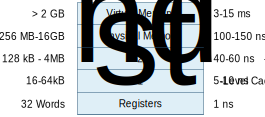
\includegraphics[width=.8\linewidth]{memory_hierarchy}
	\end{center}
\end{frame}

\begin{frame}{Locality and Memory Hierarchy}
	\begin{rightarrowsequence}
		\arrow[bg=CIADmagenta]{
			Locality permits to take advantage of the memory hierarchy
		}
		\arrow[bg=CIADlightgray,fg=black]{
			Placing the most common instructions and data in the fast-but-small storage
		}
		\arrow[bg=CIADlightgray,fg=black]{
			Leaving the rest in the slow-but-large storage
		}
		\arrow[bg=CIADgreen]{
			Minimize the average memory-access time
		}
	\end{rightarrowsequence}
\end{frame}

\begin{frame}{Optimization Policy}
	\begin{rightarrowsequence}
		\arrow[bg=CIADlightgray,fg=black]{
			Put the most-recent-used instruction in the fastest memory
		}
		\arrow[bg=CIADlightgray,fg=black]{
			Put together in the same memory page/block the instructions that may be always executed together
		}
		\arrow[bg=CIADgreen]{
			Locality of data can be improved by changing: \newline
			$1)$ the data layout \newline
			$2)$ the order of the computations
		}
	\end{rightarrowsequence}
	\begin{example}
		\begin{itemize}
			\item Visiting a large amount of data and performing small operations on it is not a good approach
			\item Preferably, smaller data should be pushed down into a faster memory level, and perform the computations on them
		\end{itemize}
	\end{example}
\end{frame}

\subsection{Allocation and deallocation}
\subsectiontableofcontentslide

\subsubsection{Chunks, holes, fragmentation, bins}

\begin{frame}{{Chunks and Holes} in the Heap}
	\begin{definitionblock}{Memory Chunk}
		A fragment of memory that is allocated and deallocated as a whole \\[.2cm]
		Size of a chunk depends on the type of object to be allocated
	\end{definitionblock}
	\vspace{.2cm}
	\begin{block}{General Principle}
		\begin{itemize}
			\item At the beginning of the program, the heap is one contiguous unit of free space
			\item As the program allocates and deallocates memory, this space is broken up into free and used chunks
		\end{itemize}
	\end{block}
	\vspace{.2cm}
	\begin{definitionblock}{Memory Hole}
		Free chunks are named hole
	\end{definitionblock}
\end{frame}

\begin{frame}{Object Placement for Minimizing the Defragmentation}
	\begin{definitionblock}{Memory Fragmentation}
		Alternating chunks and holes is named the \emph{fragmentation} of the heap
	\end{definitionblock}
	\vspace{.2cm}
	\alertbox*{
		Fragmentation is reduced by controlling how the memory manager places new objects in the heap
	}
	\vspace{.2cm}
	\titlebox*[.3\linewidth]{Best-Fit Object Placement}{
		Allocate in the smallest available hole that is large enough \newline
		\alert{Not good for spatial locality}
	}
	\hfill
	\titlebox*[.3\linewidth]{First-Fit Object Placement}{
		Allocate in the first hole, which is able to contains the requested chunk \newline
		\alert{Less efficient than the previous one}
	}
	\hfill
	\titlebox*[.3\linewidth]{Next-Fit Object Placement}{
		When no hole of the exact size was found, allocate in the lastly split hole \newline
		\alert{Good for spatial locality and efficient}
	}
\end{frame}

\begin{frame}{Bins}
	\begin{definitionblock}{Bin}
		Free space chunks are grouped into bins according to their sizes
	\end{definitionblock}
	\vspace{.2cm}
	\hiconbox{
		Many bins for the smaller sizes, because there are usually many more small objects in programs
	}{note-icon}
	\vspace{.2cm}
	\begin{alertblock}{Lea Memory Manager (GNU C compiler)}
		\begin{description}
			\item Bins of every multiple of 8 bytes until 512 bytes
			\item Larger-sized bins are logarithmically spaced
			\item Within the bins, the chunks are ordered by their sizes
			\item[Wilderness chunk] largest bin because its size may be extended after requesting more memory to OS
		\end{description}
	\end{alertblock}
\end{frame}

\subsubsection{Allocation of chunk}
\subsubsectiontableofcontentslide

\begin{frame}{Allocation of a Chunk}
	\begin{small}
		\begin{myalgorithm}
			\Inputs{Size $s$ of the chunk to be allocated; sorted list $\mathbb{S}$ of available sizes of chunks}
			\Output{Allocated chunk $c$; or error}
			\BlankLine
			\Begin{
				\If(\tcp*[f]{Search of a bin of size $s$}){$\exists c \in$bin$_s$}{
					$c$ \affect \allocate{bin$_s$} \;
					\Return{$c$}
				}
				\ForEach(\tcp*[f]{Search for smallest chunk}){$\alpha \in \mathbb{S} \cup \{\text{wilderness chunk}\}$}{
					\If{$\exists c \in$bin$_\alpha$}{
						$\langle c,r\rangle$ \affect \allocate{bin$_\alpha,s$} \tcp*{First-fit or best-fit strategy}
						$\beta$ \affect $\alpha - s$ \;
						bin$_\beta$ \affect bin$_\beta \cup r$ \;
						\Return{$c$}
					}
				}
				\throw{"Out of memory"}
			}
		\end{myalgorithm}
	\end{small}
\end{frame}

\subsubsection{Deallocation of chunk}
\subsubsectiontableofcontentslide

\begin{frame}{Deallocation and Coalescing Free Space}
	\begin{block}{Dealocation of a Chunk}
		When an object is deallocated, memory manager makes its chunk free
	\end{block}
	\vspace{.5cm}
	\begin{definitionblock}{Coalescing of Free Space}
		It may also be possible to combine (coalesce) the just freed chunk with adjacent chunks
	\end{definitionblock}
	\vspace{.5cm}
	\begin{center}
		\viconbox*[.4\linewidth]{Boundary Tags}{tag-icon}
		\hspace{1cm}
		\viconbox*[.4\linewidth]{Double-Linked Free List}{double-linked-list-icon}
	\end{center}
\end{frame}

\sidecite{Knuth.1968}
\begin{frame}{Boundary Tags}
	\begin{definitionblock}{Chunk with Boundary Tags}
		Bits of the chunk is composed by:
		\begin{itemize}
			\item \Emph{Boundary tags}
			\item Chunk data
			\item \Emph{Boundary tags} (again)
		\end{itemize}
		Order of tags depends on run-time environment
	\end{definitionblock}
	\vspace{.25cm}
	\begin{center}
		\pgfuseimage{boundary-tags}
	\end{center}
\end{frame}

\begin{frame}{Double-Linked Free List}
	\begin{small}
		\begin{definitionblock}{Free Chunks in a Double-Linked List}
			\begin{itemize}
				\item Free chunks (but not the allocated ones) are linked in a double-linked list
				\item Boundary tags include pointers to the previous and next free chunks
				\item Does not need to allocate more space for these pointers: the pointers takes the unused bytes of the free chunks
				\item For the smaller chunks, they are expanded to allow to contain the pointers
			\end{itemize}
		\end{definitionblock}
	\end{small}
	\vspace{.25cm}
	\begin{center}
		\pgfuseimage{doubly-linked-list}
	\end{center}
\end{frame}

\subsection{Manual deallocation}
\subsectiontableofcontentslide

\begin{frame}{Manual Deallocation}
	\hiconbox{
		\begin{itemize}
			\item Any storage that will no longer be accessed should be deleted
			\item Any storage that may be referenced must not be deleted
			\item \alert{It is hard to enforce these properties}
		\end{itemize}
	}{deallocation-icon}
	\vspace{.25cm}
	\hiconbox{
		Two common errors may occurs in manual memory management:
		\begin{enumerate}
			\item \alert{Memory Leak:} failing ever to delete data that cannot be referenced
			\item \alert{Dangling-pointer reference:} referencing deleted data
		\end{enumerate}
	}{danger-icon}
\end{frame}

\begin{frame}{{Memory Leak} Problem}
	\begin{small}
		\begin{block}{Observation}
			\begin{itemize}
				\item Hard for a developer to tell if a program will never refer to some storage in the future
				\item Common mistake is not deleting storage that will no more referenced
			\end{itemize}
		\end{block}
		\vspace{.25cm}
		\begin{alertblock}{Problem}
			May slow down the execution of the program due to increased memory usage
		\end{alertblock}
		\vspace{.25cm}
		\begin{block}{Remarks}
			\begin{itemize}
				\item Correctness of the program is not changed
				\item Many programs may tolerate leaks but not the long-time and critical ones (operating systems, server code\dots)
			\end{itemize}
		\end{block}
	\end{small}
\end{frame}

\begin{frame}[background=6]{Solving the Memory Leak Problem}
	\begin{enumerate}
		\item \emph{Automatic garbage collection gets rid of memory leaks by deallocating all the garbage}\\
		Even with a garbage collector, programs may still use more memory than necessary
		\vspace{1cm}
		\item \emph{A programmer may know that an object will never be referenced} \\
		He must deliberately remove the references to objects that will never be referenced, so the objects can be deallocated automatically
	\end{enumerate}
\end{frame}

\begin{frame}{Problem of Dangling-Pointer Reference}
	\begin{small}
		\begin{block}{Observation}
			\begin{itemize}
				\item Deletion of a storage, and then referencing the deleted storage
				\item These pointers are named ``dangling pointers''
			\end{itemize}
		\end{block}
		\begin{alertblock}{Problem}
			\begin{itemize}
				\item When the storage has been reallocated, it produces random effects on the program
				\item Writing through a dangling pointer changes another variable than the expecting one by the dangling pointer
			\end{itemize}
		\end{alertblock}
		\begin{block}{Remarks}
			Read, write or deallocate a pointer is named ``dereferencing the pointer''
		\end{block}
	\end{small}
\end{frame}

\begin{frame}{Solving the Dangling-Pointer-Reference Problem}
	\alertbox{Unfortunately, there is no ``magic'' solution}
	\vspace{1cm}
	\begin{enumerate}
		\item \emph{Programmer must be aware and may pay attention to his uses of the pointers}
		\vspace{.5cm}
		\item \emph{Dangling-pointer-dereference error does not occurs in run-time environments that has an \Emph{automatic garbage collector}}
	\end{enumerate}
\end{frame}

\begin{frame}{{Illegal Address} Error}
	\begin{definition}
		Occurs when the address to dereference is \ccode{null} or outside the bounds of any allocated memory (including the bounds of the memory space of the process)
	\end{definition}
	\vspace{.25cm}
	\hiconbox{
		\begin{itemize}
			\item Related to the dangling-pointer-dereference error
			\item At the origin of many security violations from hackers
		\end{itemize}
	}{note-icon}
	\vspace{.25cm}
	\begin{alertblock}{Solution}
		\begin{itemize}
			\item Compiler inserts checks with every access, to make sure it is within the bounds
			\item Compiler optimizer may remove several of these checks when they are detected as not necessary
		\end{itemize}
	\end{alertblock}
\end{frame}

\begin{frame}[t]{{Programming Conventions} and Tools}
	\begin{block}{Object Ownership}
		\begin{itemize}
			\item Associate an \Emph{owner} with each object at all times:
				\begin{itemize}
				\item Usually a function
				\item Responsible for either deleting the object or for passing the object to another owner
				\end{itemize}
			\item Non-owning pointers may reference the object, but the object must never be deallocated through them
		\end{itemize}
	\end{block}
	\vspace{.25cm}
	\hiconbox{
		\begin{itemize}
			\item Eliminates memory leaks
			\item Eliminates deletion of the same object twice
		\end{itemize}
	}{pros-icon}
	\hiconbox{
		Does not solve the dangling-point-reference problem
	}{cons-icon}
\end{frame}

\begin{frame}[t]{{Programming Conventions} and Tools \insertcontinuationtext}
	\begin{block}{Reference Counting}
		\begin{itemize}
			\item Associate a \Emph{counter} with each dynamically allocated object: \begin{itemize}
				\item counter is incremented when object is created
				\item counter is decremented when object is deleted
			\end{itemize}
			\item Object is released when the counter is zero
		\end{itemize}
	\end{block}
	\vspace{.25cm}
	\hiconbox{
		\begin{itemize}
			\item Eliminates memory leaks
			\item Eliminates deletion of the same object twice
		\end{itemize}
	}{pros-icon}
	\hiconbox{
		\begin{itemize}
		\item Expensive operation
		\item Do not work with inaccessible circular data structures
		\end{itemize}
	}{cons-icon}
\end{frame}

\begin{frame}{Programming Conventions and Tools \insertcontinuationtext}
	\begin{block}{Region-Based Allocation}
		\begin{itemize}
			\item When objects are created to be used only within some step of a computation, we can allocate all such objects in the same region
			\item Entire region is deleted once the computation step is completed
		\end{itemize}
	\end{block}
	\vspace{.25cm}
	\hiconbox{
		Very efficient
	}{pros-icon}
	\hiconbox{
		Limited applicability
	}{cons-icon}
\end{frame}

\section{Garbage collection}
\sectiontableofcontentslide

\sidecite{Wilson.1994}
\begin{frame}{Introduction to Garbage Collection}
	\alertbox*{
		\Emph{Many high-level programming languages remove the burden of manual memory management from the programmer by offering automatic garbage collection}
	}
	\vspace{.25cm}
	\begin{definitionblock}{Garbage Collection (GC)}
		Process to deallocate no-more referenced storages from the heap
	\end{definitionblock}
	\vspace{.25cm}
	\begin{itemize}
		\item First garbage collection dates from the initial implementation of LISP in 1958
		\item Several languages provide natively a GC: Java, Perl, ML, Modula-3, Prolog, Smalltalk, C\#, Ruby, Python\dots
	\end{itemize}
\end{frame}

\begin{frame}[background=6]{Hypotheses for Garbage Collection}
	\begin{enumerate}
		\item Garbage collector must know the type of the objects at run-time. This type permits to determine:
		\begin{itemize}
			\item the size of the object in bytes
			\item its components that are references to other objects
		\end{itemize}
		\vspace{.25cm}
		\item References to the objects are always to the address of the beginning of these objects
		\vspace{.25cm}
		\item All the references to the same object have the same value and may be identified easily.
	\end{enumerate}
\end{frame}

\begin{frame}{Mutator and Garbage Collection}
	\begin{definitionblock}{Mutator}
		Mutator, i.e., the \emph{user program}, modifies the collection of objects in the heap
		\begin{itemize}
			\item Creates objects by acquiring space from the memory manager
			\item Introduce and drop references to existing objects
		\end{itemize}
	\end{definitionblock}
	\vspace{1cm}
	\begin{block}{Relationship with GC}
		\begin{itemize}
			\item Objects become garbage when the mutator program cannot ``reach'' them
			\item GC finds the garbage and reclaims their space to the memory manager
		\end{itemize}
	\end{block}
\end{frame}

\subsection{Properties of a garbage collector}
\subsectiontableofcontentslide

\begin{frame}{Type Safety}
	\alertbox{Source language must be type safe}
	\hiconbox{Type of the data must be known and determined at compile or run-time}{details-icon}
	\vspace{.5cm}
	\hiconbox{GC must be able to determine if a data is a pointer to a chunk}{note-icon}
	\vspace{.25cm}
	\begin{center}
		\titlebox*[.4\linewidth]{Statically typed languages}{Types are determined at compile time (ML\dots)}
		\hspace{1cm}
		\titlebox*[.4\linewidth]{Dynamically typed languages}{Types are determined at run-time (Java\dots)}
	\end{center}
\end{frame}

\begin{frame}{Unsafe Language}
	\alertbox{\Emph{Unsafe languages (C, C++\dots) are bad candidate for GC}}
	\hiconbox{
		In unsafe languages, memory addresses can be manipulated arbitrarily (pointer arithmetic\dots) \newline
		Programs can refer to any location in memory at any time}{details-icon}
	\vspace{1cm}
	\hiconbox{
		Consequently, no memory location can be considered to be inaccessible \newline
		No storage can ever be reclaimed safely}{cons-icon}
\end{frame}

\begin{frame}{Performance Metrics}
	\hiconbox{
		\begin{minipage}{\linewidth}\begin{block}{Overall Execution Time}
			GC should not significantly increase the total run time of an application
		\end{block}\end{minipage}
		\begin{minipage}{\linewidth}\begin{block}{Pause Time}
			Simple GC causes the mutator to pause suddenly for an extremely long time. \newline
			Maximum pause time must be minimized
		\end{block}\end{minipage}
	}{gc-time-performance}
	\vspace{5cm}
	\hiconbox{
	\begin{minipage}{\linewidth}\begin{block}{Space Usage}
			GC must avoid fragmentation and make the best use of the available memory
	\end{block}\end{minipage}
	}{gc-space-performance}
\end{frame}

\begin{frame}{Performance Metrics \insertcontinuationtext}
	\hiconbox{
		\begin{minipage}{\linewidth}\begin{block}{Program Locality}
			\begin{itemize}
				\item GC speed cannot be evaluated solely by its running time
				\item GC controls the placement of data and thus influences the data locality of the mutator program
				\item GC can improve the mutator's temporal locality by freeing the space and reusing it
				\item GC can improve the mutator's spatial locality by relocating data used together in the same cache or pages
			\end{itemize}
		\end{block}\end{minipage}
	}{gc-locality-performance}
\end{frame}

\subsection{Reachability of data}
\subsectiontableofcontentslide

\begin{frame}{Root Set}
	\begin{definitionblock}{Root Set}
		It refer to all data that can be accessed directly by a program, without having to dereference any pointer
	\end{definitionblock}
	\vspace{.25cm}
	\begin{example}
		In Java, the root set is composed of all the static fields and all the variables in the stack
	\end{example}
	\vspace{.25cm}
	\begin{description}
		\item Program can \emph{reach} any member of its root set at any time
		\item Recursively, any object with a reference that is stored in the field members or array elements of any reachable object is itself reachable
	\end{description}
	\vspace{.25cm}
	\hiconbox{
		When an object becomes unreachable, it will never be reachable again
	}{note-icon}
\end{frame}

\begin{frame}{{Basic Operations} to Change the Root Set}
	\begin{block}{Object Allocation}
		\begin{itemize}
			\item Performed by the memory manager
			\item Memory manager returns a reference to each newly allocated chunk of memory
			\item This operation adds members to the set of reachable objects.
		\end{itemize}
	\end{block}
	\vspace{.5cm}
	\begin{block}{Parameter Passing and Return Values}
		\begin{itemize}
			\item References to objects are passed from the actual input parameter to the corresponding formal parameters; and from the returned result back to the caller
			\item Objects pointed by these references remain reachable
		\end{itemize}
	\end{block}
\end{frame}

\begin{frame}{{Basic Operations} to Change the Root Set \insertcontinuationtext}
	\begin{block}{Reference Assignments}
		\begin{itemize}
			\item Assignments \code{x = y} (\code{x} and \code{y} are references) have two effects:
			\begin{enumerate}
				\item \ccode{x} is a now a reference to the object referred by \ccode{y} \\
				Referenced object by \ccode{x} and \ccode{y} is reachable while \ccode{x} or \ccode{y} is reachable
				\item Original reference of \ccode{x} is lost \\
				If this lost reference is the last on the object, the object becomes unreachable
			\end{enumerate}
			\item When an object becomes unreachable, all the reachable objects inside becomes unreachable also
		\end{itemize}
	\end{block}
\end{frame}

\begin{frame}{{Basic Operations} to Change the Root Set \insertcontinuationtext}
	\begin{block}{Procedure returns}
		\begin{itemize}
			\item As a procedure exists, the activation record holding its local variables is popped off from the stack
			\item If the activation record holds the only reachable reference to any object, that object becomes unreachable
			\item If the now unreachable objects holds the only references to other objects, they become unreachable too, and so on
		\end{itemize}
	\end{block}
\end{frame}

\begin{frame}{{How Finding} Unreachable Objects?}
	\begin{block}{Approach \#1}
		\emph{Transitions from reachability to unreachability are catched}, or \\
		\emph{reachable objects are periodically located;} \\
		\emph{assuming that all the other objects are not reachable} \\[.5cm]
		Reference counting is an approximation of the first approach:
		\begin{itemize}
			\item Counter of the reference to an object is maintained
			\item When the counter goes to zero, the object becomes unreachable (discussed in the next section)
		\end{itemize}
	\end{block}
\end{frame}

\begin{frame}{{How Finding} Unreachable Objects? \insertcontinuationtext}
	\begin{block}{Approach \#2}
		\emph{Reachability is computed by tracing all the references transitively} \\[.5cm]
		\begin{itemize}
			\item Trace-based garbage collector starts by labeling/marking all objects in the root set as ``reachable''
			\item Examine iteratively all the references in reachable objects to find more reachable objects
			\item Mark the discovered objects as ``reachable''
			\item Once the reachable set is computed, GC may find the unreachable objects
			\item All the unreachable objects could be deallocated at the same time
		\end{itemize}
	\end{block}
\end{frame}

\subsection{Reference-counting garbage collector}
\subsectiontableofcontentslide

\sidenote{Collins.1960}
\begin{leftlawnframe}{Reference-Counting Garbage Collector}{gc-introduction}
	Simple and imperfect garbage collector based on reference counting \\[1cm]
	Every object must have a field for the reference counting \\
	Additional field is maintained as described in the following slides
\end{leftlawnframe}

\begin{frame}{Actions of Reference-Counting GC}
	\begin{block}{Object Allocation}
		Reference counter of the new object is \emph{set to $1$}
	\end{block}
	\vspace{.5cm}
	\begin{block}{Parameter Passing}
		Reference counter of each object passed into a procedure is \emph{incremented}
	\end{block}
	\vspace{.5cm}
	\begin{block}{Procedure Returns}
		As a procedure exists, objects referred by the local variables in its activation record have their counters \emph{decremented} \\
		If several local variables hold references to the same object, that object's counter must be decremented once for each such reference
	\end{block}
\end{frame}

 \begin{frame}{Actions of Reference-Counting GC \insertcontinuationtext}
	\begin{block}{Reference Assignment}
		For statement \ccode{u=v} (\ccode{u} and \ccode{v} are references): \\
		counter of the object referred by \ccode{v} is \emph{incremented} \\
		counter of the old object referred by \ccode{u} is \emph{decremented}
	\end{block}
	\vspace{.5cm}
	\begin{block}{Transitive Loss of Reachability}
		When the reference counter of an object \emph{becomes zero}, the counter of each object pointed by a reference within the object is \emph{decremented}
	\end{block}
\end{frame}

\begin{frame}<-11>[t,fragile]{Example of Reference-Counting Garbage Collector}
	\begin{lstlisting}[style=lststyle-java,linewidth={.4\linewidth}]
class Obj {
  public Obj a = null;
  public Obj b = null;
}

class Main {
  public static void main(String[] args) {
    Obj o1 = new Obj();
    {
      Obj o2 = new Obj();
      Obj o3 = new Obj();
      o1.b = o2;
      o2.a = o1;
      o2.b = o3;
      o3.b = o1;
    }
  }
}
	\end{lstlisting}
	\putat(180,0){\includeanimatedfigure[width=.4\paperwidth]{reference_counting_exemple}}
	\only<2>{\putat(-5,115){\pgfuseimage{rightarrow-in-code}}}
	\only<3>{\putat(0,97){\pgfuseimage{rightarrow-in-code}}}
	\only<4>{\putat(0,87){\pgfuseimage{rightarrow-in-code}}}
	\only<5>{\putat(0,77){\pgfuseimage{rightarrow-in-code}}}
	\only<6>{\putat(0,67){\pgfuseimage{rightarrow-in-code}}}
	\only<7>{\putat(0,57){\pgfuseimage{rightarrow-in-code}}}
	\only<8>{\putat(0,47){\pgfuseimage{rightarrow-in-code}}}
	\only<9>{\putat(-10,38){\pgfuseimage{rightarrow-in-code}}}
	\only<10>{\putat(-15,29){\pgfuseimage{rightarrow-in-code}}}
	\only<11>{\putat(170,190){\parbox[t]{.5\paperwidth}{\normalcolor\mdseries\small\nohyphens{
		This set of objects should be garbage collected. But their counters are greater than 0 \\
		Such a situation is tantamount to a \alert{memory leak}, since this set of objects will never be deallocated}}}}
\end{frame}

\begin{frame}<12->[t,fragile]{{Solving Memory Leak} with Reference-Counting Garbage Collector}
	\begin{lstlisting}[style=lststyle-java,linewidth={.4\linewidth}]
class Obj {
  public Obj a = null;
  public Obj b = null;
}
class Main {
  public static void main(String[] args) {
    Obj o1 = new Obj();
    {
      Obj o2 = new Obj();
      Obj o3 = new Obj();
      o1.b = o2;
      o2.a = o1;
      o2.b = o3;
      o3.b = o1;
    }
    o1.b = null;
  }
}
	\end{lstlisting}
	\putat(180,0){\includeanimatedfigure[width=.4\paperwidth]{reference_counting_exemple}}
	\only<12>{\putat(-5,48){\pgfuseimage{rightarrow-in-code}}}
	\only<12>{\putat(170,190){\parbox[t]{.5\paperwidth}{\normalcolor\mdseries\small\nohyphens{
		\alert{A line is added to reset the reference from \ccode{o1} to \ccode{o2}}}}}}
	\only<13>{\putat(-10,38){\pgfuseimage{rightarrow-in-code}}}
	\only<14>{\putat(-20,29){\pgfuseimage{rightarrow-in-code}}}
	\only<15>{\putat(170,190){\parbox[t]{.5\paperwidth}{\normalcolor\mdseries\small\nohyphens{
		Chunk, previously referred by \ccode{o2}, is no more referenced \\ It is garbage collected}}}}
	\only<16>{\putat(170,190){\parbox[t]{.5\paperwidth}{\normalcolor\mdseries\small\nohyphens{
		Chunk previously referred by \ccode{o3} is garbage collected}}}}
	\only<17>{\putat(170,190){\parbox[t]{.5\paperwidth}{\normalcolor\mdseries\small\nohyphens{
		Chunk previously referred by \ccode{o1} is garbage collected \\
		There is \Emph{no memory leak} \\[1cm]
		Weak references in several languages (e.g., Java) may be a good replacement for the added line}}}}
\end{frame}

\begin{frame}{Deferred Reference Counting}
	\begin{definition}
		Mean to eliminate the overhead associated with updating the reference counters due to stack accesses
	\end{definition}
	\vspace{1cm}
	\begin{itemize}
		\item Reference counts do not include references from the root set of the program
		\item An object is not considered to be garbage until the entire root set is scanned and no reference to the object is found
	\end{itemize}
\end{frame}

\begin{frame}[background=6]{Advantages of Reference Counting GC}
	\begin{enumerate}
		\item Garbage Collection is performed in an \emph{incremental fashion}.
		\begin{itemize}
			\item The operations are made through the mutator's operations.
			\item Removing one reference may render a large number of objects unreachable, the operation of recursively modifying reference counts can easily be deferred and performed piecemeal across time.
			\item Reference counting is particularly attractive when timing deadlines must be met.
		\end{itemize}
		\vfill
		\item Garbage are collected immediately, keeping space usage low.
	\end{enumerate}
\end{frame}

\begin{frame}[background=9]{Disadvantages of Reference Counting GC}
	\begin{enumerate}
		\item Reference counting cannot collect unreachable, cyclic data structures.
		\begin{itemize}
			\item Cyclic data structures are quite plausible.
			\item Data structures often point back to their parent nodes, or point to each other as cross references.
		\end{itemize}
		\vfill
		\item Overhead of reference counting is high:
		\begin{itemize}
			\item Additional operations were introduced with each reference assignment.
			\item Additional operations were introduced with each procedure call and exit.
			\item The overhead is proportional to the amount of computation in the program, and not just to the number of objects in the system.
		\end{itemize}
	\end{enumerate}
\end{frame}

\subsection{Trace-based garbage collector}
\subsectiontableofcontentslide

\sidecite{McCarthy.1960}
\begin{leftlawnframe}{Trace-Based Garbage Collector}{gc-introduction}
	Instead of collecting garbage as it is created, trace-based collectors run periodically to find unreachable object \\[.5cm]
	When free space is exhausted or its amount drops below a threshold \\[.5cm]
	All trace-based algorithms:
	\begin{enumerate}
		\item compute the set of reachable objects
		\item take the complement of this list
	\end{enumerate}
\end{leftlawnframe}

\subsubsection{States of the chunks}
\subsubsectiontableofcontentslide

\begin{frame}[t]{States of the Chunks}
	\vspace{-2pt}
	\begin{definitionblock}{Free}
		\begin{itemize}
			\item Chunk is in the \emph{Free} state if it is ready to be allocated
			\item Free chunk must not hold a reachable object
		\end{itemize}
	\end{definitionblock}
	\begin{definitionblock}{Allocated}
		\begin{itemize}
			\item Chunk is in the \emph{Allocated} state if it was used to store data
			\item Allocated chunk must be in one of the three substates:
			\begin{enumerate}
				\item Unreached
				\item Unscanned
				\item Scanned
			\end{enumerate}
		\end{itemize}
	\end{definitionblock}
	\begin{center}
		\pgfuseimage{chunk-states}
	\end{center}
\end{frame}

\begin{frame}[t]{States of an Allocated Chunk}
	\only<1>{\begin{definitionblock}{Unreached}
			\begin{itemize}
				\item Chunks are presumed unreachable, unless proven reachable by tracing
				\item Chunk is in the \emph{Unreached} state at any point during garbage collection if its reachability has not yet been established
				\item After a round of garbage collection, the state of a reachable object is reset to Unreachable to get ready for the next round (see the next states)
			\end{itemize}
	\end{definitionblock}}
	\only<2>{\begin{definitionblock}{Unscanned}
			\begin{itemize}
				\item Chunk is in the \emph{Unscanned} state if it is known as reachable, but its pointers have not yet been scanned
				\item Transition to Unscanned from Unreached occurs when we discover that chunk is reachable.
			\end{itemize}
	\end{definitionblock}}
	\only<3>{\begin{definitionblock}{Scanned}
			\begin{itemize}
				\item Every Unscanned object will eventually be scanned and move to the \emph{Scanned} state
				\item To scan an object, each pointer within it and follow this pointer to the target object
				\item Scanned object can only contain references to other scanned ot unscanned objects, never to unreached objects \\ $\Rightarrow$ accessible chunks are moved to the Unscanned state if they are unreachable
			\end{itemize}
	\end{definitionblock}}
	\only<4>{\begin{itemize}
			\item At the end of its algorithm, GC deallocates the unreached chunks
			\item Chunk states are set to ``Unreached'' for the next GC execution
	\end{itemize}}
	\putat*(70,-195){\includeanimatedfigure[width=.7\linewidth]{allocated_chunk_states}}
\end{frame}

\subsubsection{Basic mark-and-sweep GC}
\subsubsectiontableofcontentslide

\sidecite{McCarthy.1960}
\begin{frame}{Mark-and-Sweep GC}
	\begin{definition}
		\begin{itemize}
			\item Mark-and-sweep GC is \Emph{``stop-the-world''} algorithm
			\item Find all the unreachable objects, and put them on the list of free space
		\end{itemize}
	\end{definition}
	\vspace{1cm}
	\hiconbox{
		\begin{itemize}
			\item Visits and ``marks'' all the reachable objects in the first tracing step
			\item ``Sweeps'' the entire heap to free up unreachable objects
		\end{itemize}
	}{process-icon}
\end{frame}

\begin{frame}[t]{Algorithm of the Mark-and-Sweep Collector \insertcontinuationwith1}
	\begin{footnotesize}
		\begin{myalgorithm}
			\SetKwFunction{copyof}{copy-of}%
			\SetKwFunction{referencesin}{references\_in}%
			\Inputs{Root set of objects, a heap, and a free list (named \code{Free}), with all the unallocated chunks of the heap}
			\Output{Modified \ccode{Free} list after garbage has been removed}
			\BlankLine
			\uBegin{
				\tcc{MARKING PHASE}
				Unscanned \affect \copyof{root}\;
				\ForEach{o $\in$ Unscanned}{
					reached\_bit[o] \affect false
				}
				\While{$\exists$ o $\in$ Unscanned}{
					Unscanned \affect Unscanned $\setminus \{ o \}$\;
					\ForEach{r $\in$ \referencesin{o}}{
						\If{$neg$ reached\_bit[r]}{
							reached\_bit[r] \affect true\;
							Unscanned \affect Unscanned $\cup \{ r \}$\;
						}
					}
				}
			}
		\end{myalgorithm}
	\end{footnotesize}
\end{frame}

\begin{frame}[t]{Algorithm of the Mark-and-Sweep Collector \insertcontinuationwith2}
	\begin{footnotesize}
		\begin{myalgorithm}
			\uEnd{
				\tcc{SWEEPING PHASE}
				Free \affect $\emptyset$\;
				\ForEach{c $\in$ chunks}{
					\uIf{$neg$ reached\_bit[c]}{
						Free \affect Free $\cup \{ c \}$
					}
					\Else{
						reached\_bit[c] \affect false
					}
				}
			}
		\end{myalgorithm}
	\end{footnotesize}
\end{frame}

\begin{frame}{Optimizing Mark-and-Sweep Collector}
	\begin{alertblock}{Problem}
		\begin{itemize}
			\item Final step in the mark-and-sweep algorithm is expensive
			\item Not easy way to find unreachable objects without examining the entire heap
		\end{itemize}
	\end{alertblock}
	\vfill
	\begin{block}{Improved Algorithm}
		\begin{itemize}
			\item \Emph{Baker's Mark-and-sweep Algorithm}
			\item Keeps a list of all allocated objects
			\item Computes the difference between allocated objects and reached objects
		\end{itemize}
	\end{block}
\end{frame}

\sidecite{Baker.1992}
\begin{frame}[t]{Baker's Algorithm of the Mark-and-Sweep Collector \insertcontinuationwith1}
	\begin{footnotesize}
		\begin{myalgorithm}
			\SetKwFunction{referencesin}{references\_in}%
			\Inputs{Root set of objects, heap, free list (named \ccode{Free}), list of allocated objects \ccode{Unreached}}
			\Output{Modified \ccode{Free} and \ccode{Unreached} lists}
			\uBegin{
				\tcc{MARKING PHASE}
				Unscanned \affect $\emptyset$\;
				Scanned \affect $\emptyset$\;
				\ForEach{o $\in$ root $\cap$ Unreached}{
					Unreached \affect Unreached $\setminus \{ o \}$; Unscanned \affect Unscanned $\cup \{ o \}$\;
				}
				\While{$\exists$ o $\in$ Unscanned}{
					Unscanned \affect Unscanned $\setminus \{ o \}$\;
					Scanned \affect Scanned $\cup \{ o \}$\;
					\ForEach{r $\in$ \referencesin{o}}{
						\If{r $\in$ Unreached}{
							Unreached \affect Unreached $\setminus \{ r \}$\;
							Unscanned \affect Unscanned $\cup \{ r \}$\;
						}
					}
				}
			}
		\end{myalgorithm}
	\end{footnotesize}
\end{frame}

\sidecite{Baker.1992}
\begin{frame}[t]{Baker's Algorithm of the Mark-and-Sweep Collector \insertcontinuationwith2}
	\begin{footnotesize}
		\begin{myalgorithm}
			\uEnd{
				\tcc{SWEEPING PHASE}
				Free \affect Free $\cup$ Unreached\;
				Unreached \affect Scanned\;
			}
		\end{myalgorithm}
	\end{footnotesize}
\end{frame}

\subsubsection{Relocating collector: Mark-and-compact GC}
\subsubsectiontableofcontentslide

\begin{leftlawnframe}{Relocating Collectors}{gc-introduction}
	Move reachable objects in the heap to eliminate memory fragmentation \\[.5cm]
	After identifying holes, relocate allocated objects at one end of the heap \\
	Rest of the memory becomes a single free chunk \\[.5cm]
	Two major approaches:
	\begin{enumerate}
		\item Mark-and-compact GC
		\item Copying GC
	\end{enumerate}
\end{leftlawnframe}

\begin{frame}[background=6]{Mark-and-Compact GC}
	The mark-and-compact collector follows:
	\vfill
	\begin{enumerate}
		\item[Marking Phase] similar to the mark-and-sweep algorithms
		\vspace{.5cm}
		\item[Object Relocation] \begin{itemize}
			\item Allocated regions of the heap are scanned
			\item Address of each reachable object is computed from the low end of the heap
			\item Addresses are stored in a structure named \ccode{NewLocation}
		\end{itemize}
		\vspace{.5cm}
		\item[Object Copy] \begin{itemize}
			\item Objects are copied to their new locations
			\item References in the objects to point to are updated
		\end{itemize}
	\end{enumerate}
\end{frame}

\begin{frame}[t]{Algorithm of the Mark-and-Compact Collector \insertcontinuationwith1}
	\begin{footnotesize}
		\begin{myalgorithm}
			\SetKwFunction{copyof}{copy\_of}%
			\SetKwFunction{referencesin}{references\_in}%
			\Inputs{Root set of objects, heap, pointer marking the start of the free space (named \ccode{Free})}
			\Output{New value of pointer \ccode{Free}}
			\BlankLine
			\uBegin{
				\tcc{MARKING PHASE}
				Unscanned \affect \copyof{root}\;
				\ForEach{o $\in$ Unscanned}{
					reached\_bit[o] \affect false\;
				}
				\While{$\exists$ o $\in$ Unscanned}{
					Unscanned \affect Unscanned $\setminus \{ o \}$\;
					\ForEach{r $\in$ \referencesin{o}}{
						\If{$neg$ reached\_bit[r]}{
							reached\_bit[r] \affect true\;
							Unscanned \affect Unscanned $\cup \{ r \}$\;
						}
					}
				}
			}
		\end{myalgorithm}
	\end{footnotesize}
\end{frame}

\begin{frame}[t]{Algorithm of the Mark-and-Compact Collector \insertcontinuationwith2}
	\begin{footnotesize}
		\begin{myalgorithm}
			\SetKwFunction{sizeof}{size\_of}%
			\uBlock{
				\tcc{COMPUTE THE NEW LOCATIONS}
				NewLocation \affect $[\;]$\;
				Free \affect first address in the heap;
				\ForEach{c $\in$ chunks[0..]}{
					\If{reached\_bit[c]}{
						NewLocation[c] \affect Free\;
						Free \affect Free \sizeof{c}\;
					}
				}
			}
		\end{myalgorithm}
	\end{footnotesize}
\end{frame}

\begin{frame}[t]{Algorithm of the Mark-and-Compact Collector \insertcontinuationwith3}
	\begin{footnotesize}
		\begin{myalgorithm}
			\SetKwFunction{referencesin}{references\_in}%
			\uEnd{
				\tcc{RETARGET THE REFERENCES AND MOVE REACHED OBJECTS}
				\ForEach{c $\in$ chunks[0..]}{
					\If{reached\_bit[c]}{
						\ForEach{r $\in$ \referencesin{c}}{
							c.r \affect NewLocation[c.r]
						}
						Copy c to NewLocation[c]\;
					}
				}
				\ForEach{r $\in$ \referencesin{root}}{
					r \affect NewLocation[r]
				}
			}
		\end{myalgorithm}
	\end{footnotesize}
\end{frame}

\subsubsection{Relocating collector: Copying GC}
\subsubsectiontableofcontentslide

\sidecite{Fenichel.1969, Cheney.1970}
\begin{frame}[background=8]{Copying GC}
	\alertbox*{Copying GC reserves space to which the objects can move}
	\vspace{.5cm}
	\begin{itemize}
		\item Memory space is partitioned into two semispaces $A$ and $B$
		\item Mutator allocates in $A$ until it fill up
		\item Mutator is stopped and GC copies the reachable objects to $B$
		\item When GC finished, the roles of $A$ and $B$ are reversed
	\end{itemize}
	\vspace{.5cm}
	\alertbox*{Algorithm is proposed by C.J. Cheney \cite{Cheney.1970}}
\end{frame}

\subsubsection{Brief Comparison}
\subsubsectiontableofcontentslide

\begin{frame}[background=8]{Comparing the Costs}
	\begin{description}
		\item[Basic Mark-and-sweep] Proportional to the number of chunks in heap
		\vfill
		\item[Baker's Mark-and-sweep] Proportional to the number of reached objects
		\vfill
		\item[Basic Mark-and-compact] Proportional to the number of chunks in the heap plus the total size of the reached objects
		\vfill
		\item[Cheney's Copying Collector] Proportional to the total of the reached objects
	\end{description}
\end{frame}

\subsection{Short-pause garbage collector}
\subsectiontableofcontentslide

\begin{frame}{{Be Better Than} Trace-based Collectors}
	\begin{alertblock}{Problem of the trace-based collectors}
		\begin{itemize}
			\item Trace-based collectors do \emph{stop-the-world} GC
			\item May introduce long pauses into execution of user programs
		\end{itemize}
	\end{alertblock}
	\vspace{.5cm}
	\begin{block}{First Solution: Incremental Collection}
		Divide the work in \emph{time}, by interleaving GC and mutation
	\end{block}
	\vspace{.5cm}
	\begin{block}{Second Solution: Partial Collection}
		Divide the work in \emph{space}, by collecting a subset of the garbage at a time
	\end{block}
\end{frame}

\subsubsection{Incremental short-pause GC}
\subsubsectiontableofcontentslide

\begin{frame}[background=8]{Incremental Short-pause GC}
	\begin{alertblock}{}
		Incremental short-pause GC is conservative:
		\begin{itemize}
			\item While GC must not collect objects that are not garbage
			\item It does not have to collect all the garbage in each round
		\end{itemize}
	\end{alertblock}
	\vspace{1cm}
	\begin{itemize}
		\item Garbage left in memory is named \emph{floating garbage}
		\item Incremental GC overestimates the set of reachable objects
	\end{itemize}
\end{frame}

\begin{frame}[background=6]{Incremental Algorithm}
	\begin{enumerate}
		\item Program's root set is processed automatically, without interference with the mutator
		\vfill
		\item After finding the initial set of unscanned objects, the mutator's actions are interleaved with the tracing step
		\vfill
		\item During this period, any of the mutator's actions that may change reachability are recorded succinctly, in a side table
		\vfill
		\item Side table is used by GC to adjust the memory allocation when the mutator's actions resume their execution
		\vfill
		\item If there is not enough memory space, GC blocks the mutator until it finished to collect garbage
	\end{enumerate}
\end{frame}

\begin{frame}[background=8]{Reachable Objects}
	Set of reachable objects when tracing finished is:
	\[ \left( R \cup New \right) \setminus Lost \]
	\vfill
	\begin{itemize}
		\item $R$: set of reachable objects at the beginning of garbage collection
		\item $New$: set of allocated objects during garbage collection
		\item $Lost$:  set of objects that have become unreachable due to lost references
	\end{itemize}
\end{frame}

\begin{frame}[background=6]{Problem of the Computation of the Reachable Objects}
	\alertbox{It is expensive to compute an object's reachability every time}
	\vspace{1cm}
	\begin{itemize}
		\item Incremental GC does not attempt to collect all garbage at the end of the tracing
		\item Every garbage left behind (floating garbage) should be a subset of the Lost objects
	\end{itemize}
	\vspace{1cm}
	\[ \left( \left( R \cup New \right) \setminus Lost \right) \subseteq S \subseteq \left( R \cup New \right) \]
\end{frame}

\begin{frame}[background=8]{{Basic Incremental} Algorithm}
	\begin{itemize}
		\item First, tracing algorithm is used to find the upper bounds of $R \cup New$
		\item Mutator behavior is modified during the tracing:
		\begin{itemize}
			\item All references that existed before GC are preserved
			\item All objects created are considered reachable immediately and are placed in the Unscanned state
		\end{itemize}
		\item This scheme is conservative and finds $R$ and $New$
	\end{itemize}
	\vspace{.5cm}
	\alertbox{But the cost is high because the algorithm intercept all the write operations and remembers all the overwritten references}
	\vspace{.5cm}
	\alertbox*{Following slides proposes a solution}
\end{frame}

\sidecite{Dikjstra.1978}
\begin{frame}{Incremental Reachability Analysis}
	\begin{rightarrowsequence}
		\arrow[bg=CIADmagenta]{
			If mutator and tracing GC algorithm are interleaved, then some reachable objects may be misclassified as unreachable
		}
		\arrow{
			Because mutator may \textcolor{CIADgreen}{violate} the following invariant of GC algorithm: \newline
			Scanned object can only contain references to other scanned or unscanned objects, never unreached objects
		}
	\end{rightarrowsequence}
\end{frame}

\begin{frame}[t]{Examples of Violation}
	\begin{small}
		\begin{itemize}
			\item<1> GC finds reachable object $A$ and scans pointers within $A$, thereby putting $A$ in the Scanned state
			\item<2> Mutator stores a reference to an Unreached (but reachable) object $B$ into the Scanned object $A$. It does by copying a reference to $B$ from an object $C$ that is currently in the Unreached or Unscanned state
			\item<3> Mutator loses reference to $B$ in object $C$. It may have overwritten $C$'s reference to $B$ before the reference is scanned, or $C$ may have become unreachable and never have reached the Unscanned state to have its reference scanned
		\end{itemize}
	\end{small}
	\vspace{.5cm}
	\begin{center}
		\includeanimatedfigure[width=.8\linewidth]{violation}
	\end{center}
\end{frame}

\begin{frame}[background=8]{Avoiding the Violations}
	\begin{small}
		\begin{description}
			\item[Write Barriers] \begin{itemize}
				\item Intercepts writes of references into a Scanned object $A$
				\item When the reference is to an Unreached object $B$, then classify the object $B$ as reachable and place it in an Unscanned state
				\item or put the object $A$ in an Unscanned state
			\end{itemize}
			\item[Read Barriers] \begin{itemize}
				\item Intercept the reads of references in Unreached or Unscanned objects
				\item When the mutator reads reference to object $A$ from an object in Unreached or Unscanned state, classify $A$ as reachable and put it in the Unscanned state
			\end{itemize}
			\item[Transfer Barriers] \begin{itemize}
				\item Intercept the loss of original reference in an Unreached or Unscanned object
				\item When the mutator overwrites a reference in an Unreached or Unscanned object, save the reference being overwritten, classify it as reachable, and place the reference itself in the Unscanned state
			\end{itemize}
		\end{description}
	\end{small}
\end{frame}

\begin{frame}[background=6]{Comparison of the Mutator Barriers}
	\begin{description}
		\item[Write barriers] the most efficient of the barriers
		\vfill
		\item[Read barriers] more expensive because typically there are many more reads than there are writes
		\vfill
		\item[Transfer barriers] not competitive; because many objects ``die young,'' this approach would retain many unreachable objects
	\end{description}
\end{frame}

\subsubsection{Partial short-pause GC}
\subsubsectiontableofcontentslide

\begin{frame}{Partial Short-pause GC}
	\alertbox{Fact: ``Objects typically die young''}
	\vspace{.25cm}
	\begin{itemize}
		\item These objects becomes unreachable before the GC is invoked
		\item $\Rightarrow$ GC is cost effective with the approaches presented in the previous slides
	\end{itemize}
	\vspace{.25cm}
	\begin{itemize}
		\item The same ``mature'' objects were found and copied at every round of the GC
	\end{itemize}
	\vspace{.25cm}
	\begin{block}{Two major approaches for effective GC}
		\begin{itemize}
			\item Generational GC
			\item Train Algorithm
		\end{itemize}
	\end{block}
\end{frame}

\sidecite{Lieberman.1983}
\begin{frame}{{General Principle} of the Generational GC}
	\begin{block}{Structure}
		Heap is divided in partitions: $0$, $1$, \dots, $n$ \\
		($0$ is for the younger data)
	\end{block}
	\vspace{.5cm}
	\begin{block}{Behavior}
		\begin{itemize}
			\item Objects are created in partition $0$
			\item When the partition $0$ fills up, this participation is GC and the reachable objects are moved in partition $1$
			\item Same algorithm for partition $2$ and $3$, \dots $n-1$ and $n$
		\end{itemize}
	\end{block}
\end{frame}

\sidecite{Hudson.1992}
\begin{frame}{Car and Train Definitions}
	\alertbox*{Train algorithm uses fixed-length partitions, called \emph{cars}}
	\vspace{.5cm}
	\begin{definitionblock}{Car}
		Car is a single disk block, assuming there are no object larger than disk blocks \\
		OR \\
		Car size could be larger, but it is fixed once and for all
	\end{definitionblock}
	\vspace{.5cm}
	\begin{definitionblock}{Train}
			Cars are organized into trains \\[.2cm]
			No limit to the number of cars in a train \\
			No limit to the number of trains
	\end{definitionblock}
\end{frame}

\begin{frame}{{General Principles} of the Train Algorithm}
	\alertbox*{Two approaches to collect the garbages}
	\vspace{.25cm}
	\begin{enumerate}
		\item<1> First car in lexicographic order is collected in one incremental garbage-collection step: \begin{itemize}
			\item Step similar to collection of the first partition in the generational algorithm, since a ``remembered'' list of all points from outside the car is maintained
			\item Objects with no references at all are identified, as well as garbage cycles that are contained completely within this car
			\item Reachable objects in the car are always moved to some other car, so each garbage-collected car becomes empty and can be removed from the train
		\end{itemize}
		\item<2> Sometimes, the first train has no external reference \begin{itemize}
			\item There are no pointer from the root set to any car of the train, and the remembered sets for the cars contain only references from other cars in the train, not from other trains
			\item In this situation, the train is a huge collection of cyclic garbage, and we delete the entire train
		\end{itemize}
	\end{enumerate}
\end{frame}

\begin{frame}[background=6]{{Generational GC} vs. Train Algorithm}
	\begin{itemize}
		\item Generational GC works most frequently on the area of the heap that contains the youngest objects \\
		It tends to collect a lot of garbage for relatively little work
		\vfill
		\item Train algorithm does not spend a large proportion of time on young objects \\
		It does limit the pauses due to garbage collection \\
		Advantage is that we never have to do a complete garbage collection, as we do occasionally for generational garbage collection
		\vfill
		\item Good combination of strategies is to use generational collection  for young objects, and once heap becomes sufficiently mature, to ``promote'' it to a separate heap that is managed by the train algorithm
	\end{itemize}
\end{frame}

\section{Conclusion}
\sectiontableofcontentslide

\begin{frame}{{Key Concepts} in the Chapter}
	\begin{description}
		\item[Run-time Organization] To implement the abstractions embodied in the source language, a compiler creates and manages a run-time environment in concert with the operating system and the target machine. The run-time environment has static data areas for the object code and the static data objects created at compile time. It also has dynamic stack and heap areas for managing objects created and destroyed as the target program executes
		\item[Control Stack]  Procedure calls and returns are usually managed by a run-time stack called the \emph{control stack}. We can use a stack because procedure calls or \emph{activations} nest in time; that is, if \ccode{p} calls \ccode{q}, then this activation of \ccode{q} is nested within this activation of \ccode{p}
	\end{description}
\end{frame}

\begin{frame}{{Key Concepts} in the Chapter \insertcontinuationtext}
	\begin{description}
		\item[Stack Allocation] Storage for local variables can be allocated on a run-time stack for languages that allow or require local variables to become inaccessible when their procedures end. For such languages, each live activation has an \emph{activation record} (or \emph{frame}) on the control stack, with the root of the activation tree at the bottom, and the entire sequence of activation records on the stack corresponding to the path in the activation tree to the activation where control currently resides. The latter activation has its record at the top of the stack
		\item[Access to Nonlocal Data on the Stack] For languages like C that do not allow nested procedure declarations, the location for a variable is either global or found in the activation record on top of the run-time stack. For languages with nested procedures, we can access nonlocal data on the stack through \emph{access links}, which are pointers added to each activation record. The desired nonlocal data is found by following a chain of access links to the appropriate activation record. A \emph{display} is an auxiliary array, used in conjunction with access links, that provides an efficient short-cut alternative to a chain of access links
	\end{description}
\end{frame}

\begin{frame}{{Key Concepts} in the Chapter \insertcontinuationtext}
	\begin{description}
		\item[Heap Management] The \emph{heap} is the portion of the store that is used for data that can live indefinitely, or until the program deletes it explicitly. The \emph{memory manager} allocates and deallocates space within the heap. \emph{Garbage collection} finds spaces within the heap that are no longer in use and can therefore be reallocated to house other data items. For languages that require it, the garbage collector is an important subsystem of the memory manager
		\item[Exploiting Locality] By making good use of the memory hierarchy, memory managers can influence the run time of a program. The time taken to access different parts of memory can vary from nanoseconds to milliseconds. Fortunately, most programs spend most of their time executing a relatively small fraction of the code and touching only a small fraction of the data. A program has \emph{temporal locality} if it is likely to access to same memory locations again soon; it has \emph{spatial locality} if it is likely to access nearby memory locations soon
	\end{description}
\end{frame}

\begin{frame}{{Key Concepts} in the Chapter \insertcontinuationtext}
	\begin{description}
		\item[Reducing Fragmentation] As the program allocates and deallocates memory, the heap may get \emph{fragmented}, or broken into large numbers of small noncontiguous free spaces or holes. The best fit strategy (allocate the smallest available hole that satisfies a request) has been found empirically to work well. While best fit tends to improve space utilization, it may not be best for spatial locality. Fragmentation can be reduced by combining or \emph{coalescing} adjacent holes
		\item[Manual Deallocation] Manual memory management has two common failings: not deleting data that can not be referenced is a \emph{memory-leak} error, and referencing deleted data is a \emph{dangling-pointer-reference} error
		\item[Reachability] \emph{Garbage} is data that cannot be referenced or reached. There are two basic ways of finding unreachable objects: either catch the transition as a reachable object turns unreachable, or periodically locate all the reachable objects and infer that all remaining objects are unreachable
	\end{description}
\end{frame}

\begin{frame}{{Key Concepts} in the Chapter \insertcontinuationtext}
	\begin{description}
		\item[Reference-Counting Collectors] maintain a count of the references to an object; when the count transitions to zero, the object becomes unreachable. Such collectors introduce the overhead of maintaining references and can fail to find ``cyclic'' garbage, which consists of unreachable objects that reference each other, perhaps through a chain of references
		\item[Trace-Based Garbage Collectors] iteratively examine or trace all references to find reachable objects, starting with the \emph{root set} consisting of objects that can be accessed directly without having to dereference any pointers
		\item[Mark-and-Sweep Collectors] visit and mark all reachable objects in a first tracing step and then sweep the heap to free up unreachable objects
		\item[Mark-and-Compact Collectors] improve upon mark-and-sweep; they \emph{relocate} objects in the heap to eliminate memory fragmentation
	\end{description}
\end{frame}

\begin{frame}{{Key Concepts} in the Chapter \insertcontinuationtext}
	\begin{description}
		\item[Copying Collectors] break the dependency between tracing and finding free space. They partition the memory into two \emph{semispaces}, A and B. Allocation requests are satisfied from one semispace, say A, until it fills up, at which point the garbage collector takes over, copies the reachable objects to the other space, say B, and reverses the roles of the semispaces
		\item[Incremental Collectors] Simple trace-based collectors stop the user program while garbage is collected. \emph{Incremental collectors} interleave the actions of the garbage collector and the \emph{mutator} or user program. The mutator can interfere with incremental reachability analysis, since it can change the references within previously scanned objects. Incremental collectors therefore play it safe by overestimating the set of reachable objects; any ``floating garbage'' can be picked up in the next round of collection
	\end{description}
\end{frame}

\begin{frame}{{Key Concepts} in the Chapter \insertcontinuationtext}
	\begin{description}
		\item[Partial Collectors] also reduce pauses; they collect a subset of the garbage at a time. The best known of partial-collection algorithms, \emph{generational garbage collection}, partitions objects according to how long they have been allocated and collects the newly created objects more often because they tend to have shorter lifetimes. An alternative algorithm, the \emph{train algorithm}, uses fixed length partitions, called cars, that are collected into \emph{trains}. Each collection step is applied to the first remaining car of the first remaining train. When a car is collected, reachable objects are moved out to the other cars, so this car is left with garbage and can be removed from the train. These two algorithms can be used together to create a partial collector that applies the generational algorithm to younger objects and the train algorithm to more mature objects
	\end{description}
\end{frame}

\begin{frame}[t,fancyframetitle=false,allowframebreaks]{\bibname\ of the Chapter}%
	\tiny%
	\putbib[chapters/chapter5/biblio]%
\end{frame}%

\end{bibunit}
\end{graphicspathcontext}

\endinput
